This literature review examines recent work in retail shelf monitoring, computer vision for inventory detection, and alerting systems for store automation.

\section{Retail Shelf Monitoring}

Automated shelf monitoring has become an important research area in retail analytics. Early systems used barcode scanning and RFID tags to track inventory, but these approaches require tags on every product and do not measure physical shelf occupancy directly. More recent solutions rely on image-based monitoring to detect whether products are present on shelves and to infer stock levels without modifying packaging.
\\
Research by Li et al. (2022) demonstrates that camera-based shelf monitoring can detect empty display segments with high accuracy in supermarket settings. Their work uses deep learning models to segment shelf regions and identify missing products, achieving robust performance under varied lighting and shelf layouts.

\section{Computer Vision for Product Detection}

Object detection models such as YOLO, Faster R-CNN, and SSD are widely applied in retail inventory problems. YOLOv5 and YOLOv8 are especially popular because they provide real-time performance with acceptable accuracy on edge devices.
\\
Product detection in retail is challenging due to occlusion, small objects, and dense arrangements. Huang et al. (2023) compare one-stage and two-stage detectors for shelf item recognition and show that one-stage detectors are more suitable for real-time stock monitoring, while two-stage detectors can improve accuracy for small items.

\section{Shelf Occupancy and Restocking Alerts}

Shelf occupancy estimation focuses on determining whether a given shelf location is filled or empty, rather than identifying every product that is present. This simplifies the problem and allows systems to generate actionable alerts quickly.
\\
A common approach is to divide the shelf into fixed slots or regions and use occupancy classifiers to mark each region as occupied or empty. This method is effective in grocery stores where products are arranged in consistent columns or vertical slots.
\\
Alert systems may combine occupancy information with time-based thresholds. For example, if a region remains empty for longer than a configured interval, the system flags it for restocking. This reduces the need for continuous manual inspection.

\section{Edge Deployment and Real-Time Processing}

Commercial shelf monitoring systems often deploy models at the edge to avoid latency and preserve privacy. Edge devices capture video frames, run detection locally, and send only summary status updates to the store dashboard.
\\
Edge deployment requirements include lightweight models, efficient image preprocessing, and robustness to environmental variation. Recent work by Patel and Kumar (2024) shows that compact models such as MobileNet and YOLO-tiny can deliver adequate shelf monitoring performance while running on low-cost hardware.

\section{Summary of Gaps}

Existing solutions are effective for large supermarket aisles, but many small retail stores still lack practical and affordable shelf monitoring systems. Key gaps include:
\begin{itemize}
    \item Limited support for mixed product arrangements and small shelf sections.
    \item Insufficient real-time alerting tailored to store staff workflows.
    \item High cost or complexity of commercial retail monitoring offerings.
\end{itemize}

\begin{figure}[H]
    \centering
    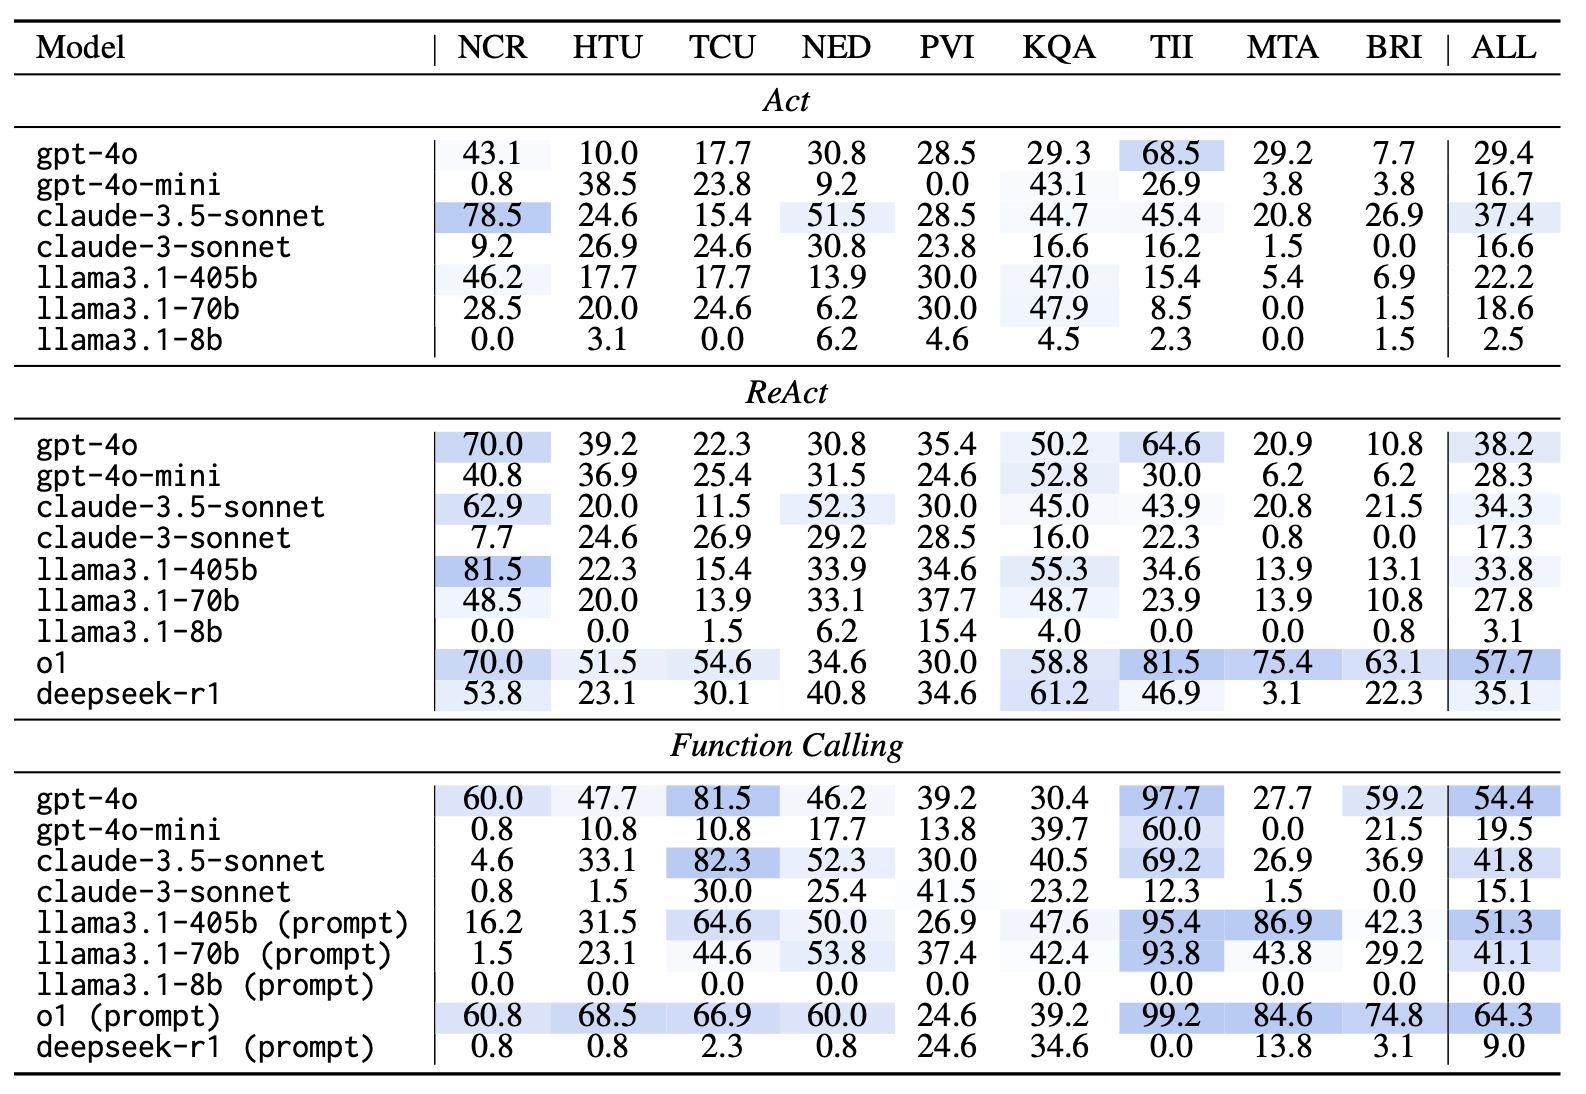
\includegraphics[width=0.8\textwidth]{figures/review/CRM_Performance.png}
    \caption{Literature Comparison (Placeholder - to be added)}
    \label{fig:literature-comparison}
\end{figure}

This project addresses these gaps by developing a lightweight system for real-time shelf occupancy monitoring and alert generation, aligned with Multinet's retail automation objectives.
